
\documentclass[../notes.tex]{subfiles}

\graphicspath{{\subfix{../img/}}}

\begin{document}

\section{ECE353 Operating Systems}

\subsection{Kernel Mode}
\subsubsection{ISAs and Permissions}

There are a number of ISAs in use today; x86 (amd64), aarch64 (arm64), and risc-v are common ones.
For purposes of this course we will study largely arm systems but will touch on the other two as well.

\begin{figure}[H]
  \centering
  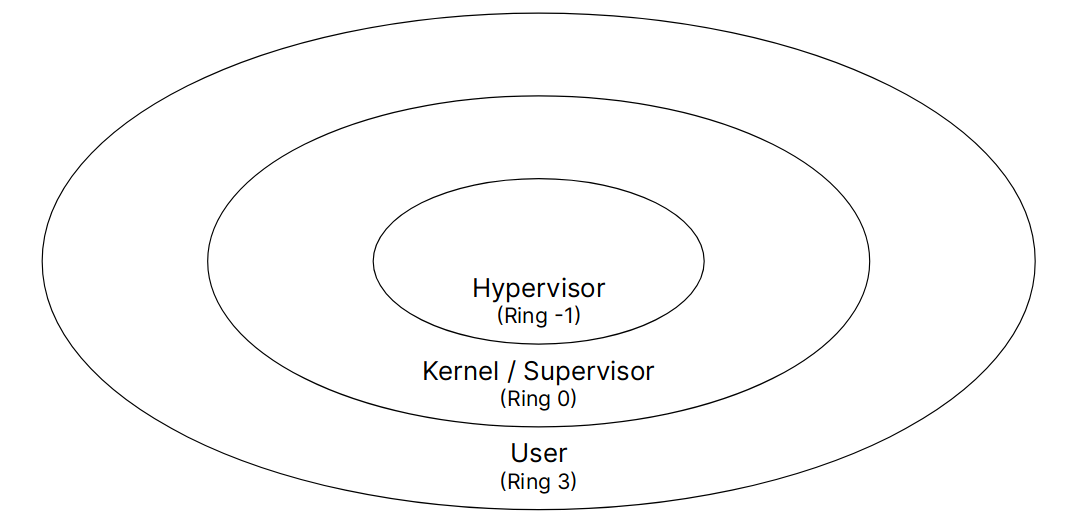
\includegraphics[width=0.8\linewidth]{img/image_2023-01-11-15-18-10.png}
  \caption{x86 Instruction access rings. Each ring can access instructions in its outer rings.}
\end{figure}

The kernel runs in, well, Kernel mode. \textbf{System calls} offer an interface between user and kernel mode\mn{Linux has 451 total syscalls}. 

\marginnote{Note: API (application programming interface), ABI (Application Binary Interface). API abstracts communication interface (i.e. two ints), ABI is how to layout data, i.e. calling convention}

The system call ABI for x86 is as follows:

\begin{figure}[H]
  \centering
  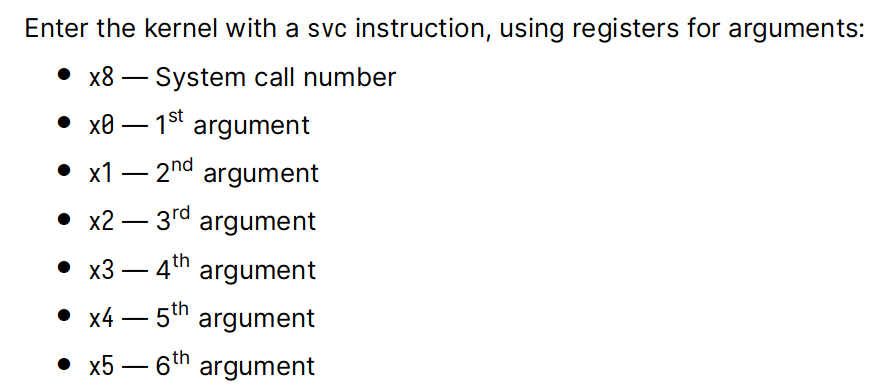
\includegraphics[width=0.8\linewidth]{img/image_2023-01-11-15-23-26.png}
\end{figure}

This ABI has some limitations; i.e. all arguments must be a register in size and so forth, which we generally circumvent by using pointers.

For example, the \texttt{write} syscall can look like:


\begin{listing}[H]
\begin{minted}{c}
ssize_t write(int fd, const void* buf, size_t count);
// writes bytes to a file descriptior
\end{minted}
\end{listing}


\subsubsection{ELF (Executable and Linkable Format)}


\begin{itemize}
  \item  Aways starts with 4 bytes: \texttt{0x7F, 'E', 'L', 'F'}
  \item Followed byte for 32 or 64 bit architecture
  \item Followed by 1 byte for endianness
\end{itemize}
\marginnote{Most file formats have different starting signatures or magic numbers}

\texttt{readelf} can be used to read \texttt{ELF} file headers.

For example, \texttt{readelf -a \$(which cat)} produces (output truncated)



\begin{listing}[H]
\begin{minted}{text}
ELF Header:
  Magic:   7f 45 4c 46 02 01 01 00 00 00 00 00 00 00 00 00
  Class:                             ELF64
  Data:                              2's complement, little endian
  Version:                           1 (current)
  OS/ABI:                            UNIX - System V
  ABI Version:                       0
  Type:                              DYN (Position-Independent Executable file)
  Machine:                           Advanced Micro Devices X86-64
  Version:                           0x1
  Entry point address:               0x32e0
  Start of program headers:          64 (bytes into file)
  Start of section headers:          33152 (bytes into file)
  Flags:                             0x0
  Size of this header:               64 (bytes)
  Size of program headers:           56 (bytes)
  Number of program headers:         13
  Size of section headers:           64 (bytes)
  Number of section headers:         26
  Section header string table index: 25
\end{minted}
\end{listing}
\marginnote{This output is followed by information about the program and section headers}


\texttt{strace} can be used to trace systemcalls. For example let's look at the 168-byte hello-world example


\begin{listing}[H]
\begin{minted}{text}
0x7F 0x45 0x4C 0x46 0x02 0x01 0x01 0x00 0x00 0x00 0x00 0x00 0x00 0x00 0x00 0x00
0x02 0x00 0xB7 0x00 0x01 0x00 0x00 0x00 0x78 0x00 0x01 0x00 0x00 0x00 0x00 0x00
0x40 0x00 0x00 0x00 0x00 0x00 0x00 0x00 0x00 0x00 0x00 0x00 0x00 0x00 0x00 0x00
0x00 0x00 0x00 0x00 0x40 0x00 0x38 0x00 0x01 0x00 0x40 0x00 0x00 0x00 0x00 0x00
0x01 0x00 0x00 0x00 0x05 0x00 0x00 0x00 0x00 0x00 0x00 0x00 0x00 0x00 0x00 0x00
0x00 0x00 0x01 0x00 0x00 0x00 0x00 0x00 0x00 0x00 0x01 0x00 0x00 0x00 0x00 0x00
0xA8 0x00 0x00 0x00 0x00 0x00 0x00 0x00 0xA8 0x00 0x00 0x00 0x00 0x00 0x00 0x00
0x00 0x10 0x00 0x00 0x00 0x00 0x00 0x00 0x08 0x08 0x80 0xD2 0x20 0x00 0x80 0xD2
0x81 0x13 0x80 0xD2 0x21 0x00 0xA0 0xF2 0x82 0x01 0x80 0xD2 0x01 0x00 0x00 0xD4
0xC8 0x0B 0x80 0xD2 0x00 0x00 0x80 0xD2 0x01 0x00 0x00 0xD4 0x48 0x65 0x6C 0x6C
0x6F 0x20 0x77 0x6F 0x72 0x6C 0x64 0x0A
\end{minted}
\caption{Note: This is for arm cpus}
\end{listing}


If we run this then we see that the program makes a \texttt{write} syscall as well as a \texttt{exit\_group}

\begin{listing}[H]
\begin{minted}{text}
execve (" ./ hello_world " , [ " ./ hello_world " ] , 0 x7ffd0489de40 /* 46 vars */ ) = 0
write (1 , " Hello world \ n " , 12) = 12
exit_group (0) = ?
+++ exited with 0 +++
\end{minted}
\end{listing}

Note that these strings are not null-terminated (null-termination is just a \texttt{c} thing) because we don't want to be unable to write strings with the null character to it.


\begin{figure}[H]
  \centering
  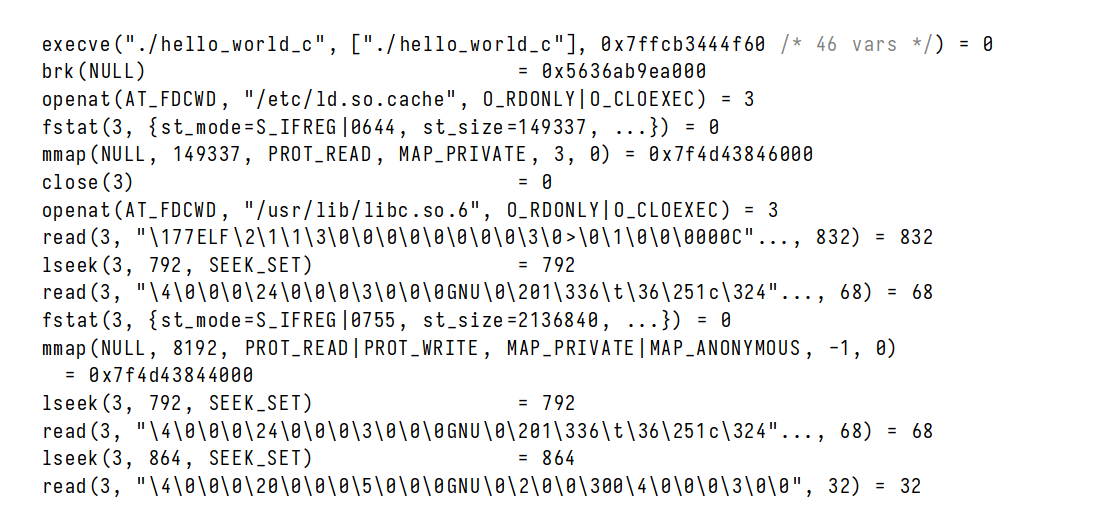
\includegraphics[width=0.8\linewidth]{img/image_2023-01-11-15-48-48.png}
  \caption{A c hello world would load the stdlib before printing...}
\end{figure}


\subsubsection{Kernel}
The kernel can be thought of as a long-running program with a ton of library code which executes on-demand. Monolithic kernels run all OS services in kernel mode, but micro kernels run the minimum amount of servers in kernel mode. Syscalls are slow so it can be useful to put things in the kernel space to make it faster. But there are security reasons against putting everything in kernel mode.


\subsubsection{Processes & Syscalls}

A process is like a combination of all the virtual resources; a "virtual GPU" (if applicable), memory (addr space), I/O, etc.
The unique part of a struct is the PCB (Process Control Block) which contains all of the execution information. In Linux this is the \texttt{task_struct} which contains information about the process state, CPU registers, scheduling information, and so forth.


\begin{figure}[H]
  \centering
  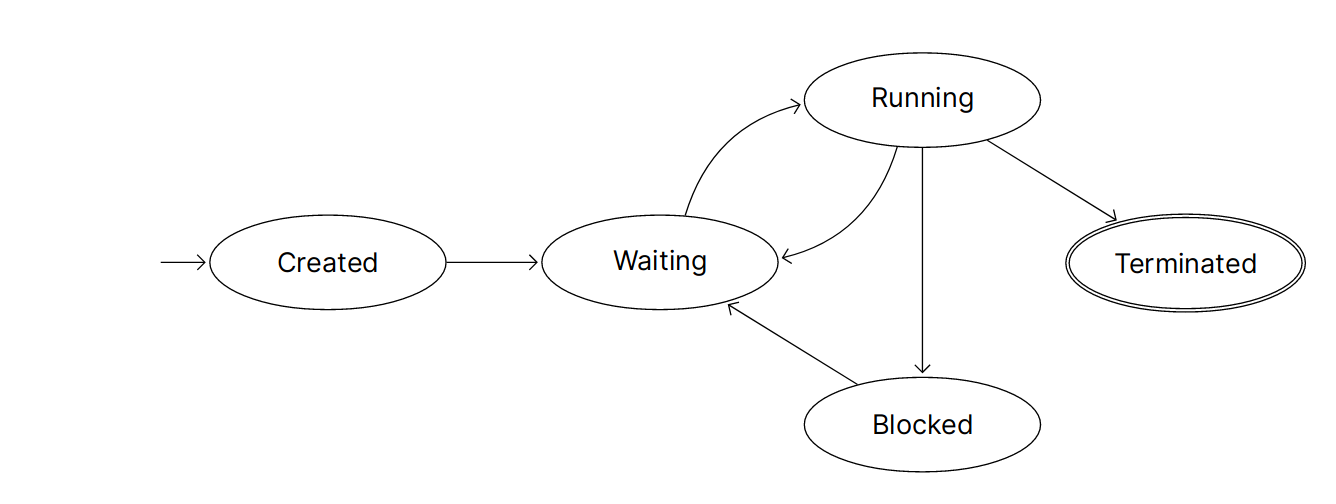
\includegraphics[width=0.8\linewidth]{img/image_2023-01-12-15-21-01.png}
  \caption{A possible process state diagram}
\end{figure}

These state changes are managed by the Process and OS\mn{I think} so that the OS scheduler can do its job.
An example of where some of these states can be useful would be to free up CPU time while a process is in the Blocked state while waiting for IO.
Process can either manage themselves (cooperative multitasking) or have the OS manage it (true multitasking).
Most systems use a combination of the two, but it's important to note that cooperative multitasking is not true multitasking.

\marginnote{Process state can be read in \texttt{/proc} for linux systems. }


Context switching (saving state when switching between processes) is expensive. Generally we try to minimize the amount of state that has to be saved (the bare minimum is the registers).
The scheduler decides when to switch. Linux currently uses the CFS\mn{completely fair scheduler}.


In \texttt{c} most system calls are wrapped to give additional features and to put them more concretely in the userspace.


\begin{figure}[H]
  \centering
  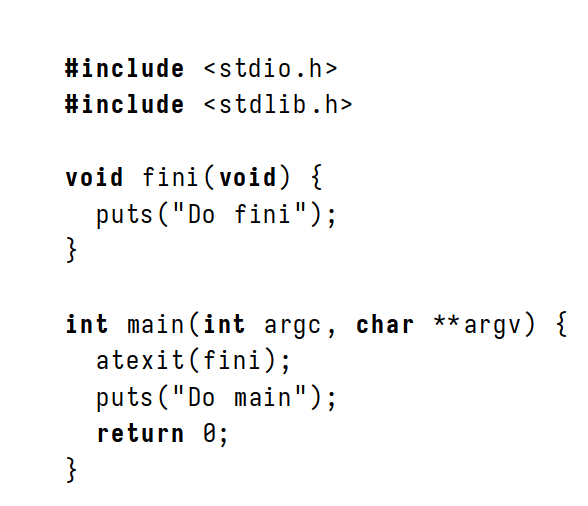
\includegraphics[width=0.8\linewidth]{img/image_2023-01-12-15-34-58.png}
  \caption{Demonstration of c feature to register functions to call on program exit}
\end{figure}

\begin{listing}[H]
\begin{minted}{c}
int main ( int argc , char * argv []) {
  printf ("I 'm going to become another process \n" );
  char * exec_argv [] = {" ls " , NULL };
  char * exec_envp [] = { NULL };
  int exec_return = execve ("/ usr / bin / ls " , exec_argv , exec_envp );
  if ( exec_return == -1) {
    exec_return = errno ;
    perror (" execve failed " );
    return exec_return ;
  }
  printf (" If execve worked , this will never print \n" );
  return 0;
}
\end{minted}
\caption{Demo of execve turning current program to ls (executes program, wrapper around exec syscall)}
\end{listing}

\begin{listing}[H]
\begin{minted}{c}
#include <sys/syscall.h>
#include <unistd.h>

int main (){
  syscall(SYS_exit_group, 0);
}

\end{minted}
\caption{An example of using a raw syscall system exit instead of c's exit()}
\end{listing}




\end{document}
